\documentclass{beamer}

\input{../../spec_files/course_preamble.tex}
\subtitle{Foundations of Neuro-Symbolic AI}
\date{Summer Term 2026}
\author[FONS]{Alex Goessmann}
\institute[]{
    University of Applied Science Würzburg-Schweinfurt
%    Weierstrass Institute for Applied Analysis and Stochastic
}

%\newcommand{\techwstitle}{
%\small
%%Workshop \\
%Logik für Erklärbare KI:
%Technische Einführung in das ENEXA Projekt}
%\newcommand{\smalltechwstitle}{ENEXA Workshop}

%\newcommand{\techwsdate}{15.+16. July, 2024}

%\newcommand{\techwsauthors}{
%Alex Goessmann
%}

%\newcommand{\techwsinclude}{
%	\usepackage{../../spec/beamercolorthemeclaw}
%	\usepackage{/Users/alexgoessmann/Documents/ENEXA/latex_macros/beamer_template/beamerfontthemeclaw}
%	\usepackage{/Users/alexgoessmann/Documents/ENEXA/latex_macros/beamer_template/beamerinnerthemeclaw}
%	\usepackage{/Users/alexgoessmann/Documents/ENEXA/latex_macros/beamer_template/beamerouterthemeclaw}
%
%	\input{/Users/alexgoessmann/Documents/ENEXA/latex_macros/packages.tex}
%	\input{/Users/alexgoessmann/Documents/ENEXA/latex_macros/macros.tex}
%	\input{/Users/alexgoessmann/Documents/ENEXA/latex_macros/macros_tc.tex}
%	\input{/Users/alexgoessmann/Documents/ENEXA/latex_macros/tikz_blocks.tex}
%
%	\subtitle{\techwstitle}
%	\date[\techwsdate]{\techwsdate}
%	\author[\smalltechwstitle]{\techwsauthors}
%	\institute[]{\eupic}
%}

\newcommand{\techwschapterone}{I-Tensors}
\newcommand{\techwschaptertwo}{II-Probabilities}
\newcommand{\techwschapterthree}{III-Logics}
\newcommand{\techwschapterfour}{IV-Applications}

\newcommand{\eupic}{
\begin{center}
	%\includegraphics[width=4cm]{/Users/alexgoessmann/Documents/ENEXA/latex_macros/images/fundedEU.png}
\end{center}
}

\newcommand{\enexadateveublock}{
\begin{center}\begin{tikzpicture}
  	%\node [anchor=center] at (0,0) {\includegraphics[width = 1.5cm]{/Users/alexgoessmann/Documents/ENEXA/latex_macros/images/DATEV.png}};
	%\node [anchor=center] at (2.5,0.5) {\includegraphics[width = 3.5cm]{/Users/alexgoessmann/Documents/ENEXA/latex_macros/images/enexa.png}};
	%\node [anchor=center] at (2.55,-0.5) {\includegraphics[width = 3cm]{/Users/alexgoessmann/Documents/ENEXA/latex_macros/images/fundedEU.png}};
\end{tikzpicture}\end{center}
}


%% OLD
\newcommand{\aselectionvariable}{L}
\newcommand{\vselectionvariable}{L}
\newcommand{\fselectionvariable}{L}
\newcommand{\cselectionvariable}{L}
\newcommand{\individualorder}{n}
\newcommand{\variableof}[1]{\indvariableof{#1}}
\newcommand{\sindex}{s}
\newcommand{\pindex}{p}
\newcommand{\oindex}{o}
\newcommand{\exquery}{q}
%\newcommand{\datapointof}[1]{x^{#1}}
\newcommand{\atomicqueryof}[1]{g_{#1}}
\newcommand{\facsystem}{\shortcatvariables}
\newcommand{\margprobof}[1]{\probat{#1}}
\newcommand{\mlnprobabilityof}[1]{\expdistof{#1}}
%\newcommand{\oldenexadateveublock}{
%	\begin{center}
%	\begin{minipage}{0.2\textwidth}
%		\begin{center}
%			\includegraphics[width = 2.5cm]{images/DATEV.png}
%		\end{center}
%	\end{minipage}
%	\begin{minipage}{0.55\textwidth}
%		\begin{center}
%			\includegraphics[width=5.5cm]{images/enexa.png} \\
%			\includegraphics[width=5.5cm]{images/fundedEU.png} \\
%		\end{center}
%	\end{minipage}
%	\end{center}
%}

\title[Models for KGs]{
	\techwschapterfour \\
	{\huge Statistical Models of Knowledge Graphs}
}
\usepackage{algorithmic}
\begin{document}

{\frame[plain]{\titlepage}}



%% From THWS Kolloquium
\newcommand{\stanspace}{\hspace{0.5cm}\\}
\newcommand{\urisize}{\small}
\newcommand{\rdfscolor}{magenta}
\newcommand{\rdfcolor}{red}
\newcommand{\owlcolor}{blue}
\newcommand{\rulecolor}{black!40!green}
\newcommand{\eqspace}{\quad\quad\quad}







\begin{frame}{Knowledge Graphs: Data stored in Graphs}

Resource Description Framework (RDF):
\begin{itemize}
\item Data is stored in form of triples (Subject,Predicate,Object)
\only<2-3>{
\item All entities are described by Uniform Resource Identifiers (URI), using prefix notation (e.g.: loc)
}
\end{itemize}
\begin{center}
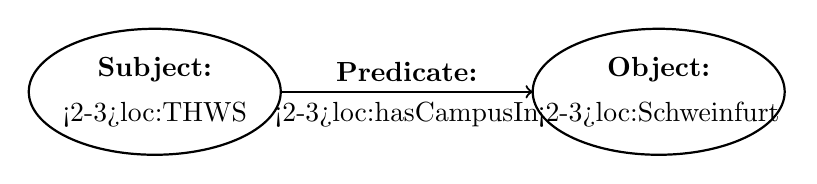
\begin{tikzpicture}[thick,scale=0.8]
	\draw (0,0) ellipse (2 and 1) node[above] {\textbf{Subject:}} 
							node[below] {\only<2-3>{loc:}THWS};
	\draw[->] (2,0) -- (6,0)  node[midway,above] {\textbf{Predicate:}} node[midway,below] {\only<2-3>{loc:}hasCampusIn};
	\draw (8,0) ellipse (2 and 1) node[above] {\textbf{Object:}} 
							node[below] {\only<2-3>{loc:}Schweinfurt};
\end{tikzpicture}
\end{center}

\only<3>{
Representation in Turtle syntax:\\
\medskip
$\mathrm{@prefix} \quad   \mathrm{loc}$:$ \quad  \mathrm{<www.locationdemo.de/location/ontology \# >} \quad  . $  \\
\medskip
$\mathrm{loc}$:$\mathrm{THWS} \quad \mathrm{loc}$:$\mathrm{hasCampusIn} \quad  \mathrm{loc}$:$\mathrm{Schweinfurt} \quad .$
}

\end{frame}


\begin{frame}{RDF, RDFS and OWL: Relation to Formal Logic}

%}-\mathrm{
$\mathrm{@prefix} \quad \mathrm{rdf:} \quad <\text{http://www.w3.org/1999/02/22-rdf-syntax-ns\#}>  .$
$\mathrm{@prefix} \quad \mathrm{rdfs:} \quad <\text{http://www.w3.org/2000/01/rdf-schema\#}> .$
$\mathrm{@prefix} \quad \mathrm{owl:} \quad <\text{http://www.w3.org/2002/07/owl\# }>.$\\

\stanspace

\textcolor{\rdfcolor}{RDF} and \textcolor{\rdfscolor}{RDF Schema (RDFS)}:
\begin{itemize}
	\item {\bf Class memberships:} $\mathrm{City(Schweinfurt)}$ \\
		$\eqspace \mathrm{loc:Schweinfurt} \quad \textcolor{\rdfcolor}{\mathrm{rdf:type}}  \quad \mathrm{{loc:City}}  \quad .$
	\item {\bf Subclass hierarchies:} $\forall x : \mathrm{City} (x) \rightarrow \mathrm{Location}(x)$ \\
		$\eqspace \mathrm{loc:City} \quad \textcolor{\rdfscolor}{\mathrm{rdfs:subClassOf}}  \quad \mathrm{loc:Location} \quad . $
\end{itemize}

\stanspace

\textcolor{\owlcolor}{Web Ontology Language (OWL)}
\begin{itemize}
	\item {\bf Classes:} $\mathrm{Class(City)}$ \\
		$ \eqspace \mathrm{loc:City} \quad \textcolor{\rdfcolor}{\mathrm{rdf:type}}  \quad \textcolor{\owlcolor}{\mathrm{owl:Class}}  \quad . $
	\item {\bf Object properties:} $\mathrm{Property(hasCampusIn)}$ \\
		$ \eqspace \mathrm{loc:hasCampusIn} \quad \textcolor{\rdfcolor}{\mathrm{rdf:type}} \quad \textcolor{\owlcolor}{\mathrm{owl:ObjectProperty}} \quad . $
\end{itemize}
%\end{spacing}
\end{frame}


\begin{frame}{Inference Example: \\
RDFS Subclass Relation}

\begin{center}
\begin{tikzpicture}[scale=0.55,thick]

	\draw (8,0) ellipse (2 and 1) node[] {\urisize loc:Schweinfurt};	
	\textcolor{\rdfcolor}{
	\draw[->] (10,0) -- (14,0)  node[midway,above] {\urisize \textcolor{\rdfcolor}{rdf:type}};}
	\draw (16,0) ellipse (2 and 1) node[] {loc:City};
	\textcolor{\rdfcolor}{
	\draw[->] (18,0) -- (22,0)  node[midway,above]  {\urisize rdf:type};
	} 
	\textcolor{\owlcolor}{
	\draw (24,0) ellipse (2 and 1) node[] {\urisize owl:Class};	}

	\textcolor{\rdfscolor}{
	\draw[->] (16,-1) -- (16,-2)  node[midway,right] {\urisize rdfs:subClassOf};}
	\draw (16,-3) ellipse (2 and 1) node[] {\urisize loc:Location};	
	\textcolor{\rdfcolor}{
	\draw[->] (18,-3) -- (24,-1)  node[midway,right]  {\urisize rdf:type};
	} 
	
	\only<3>{
	\textcolor{\rulecolor}{
	\draw[thick,->] (8,-1) -- (14,-3) node[midway,left] {\urisize rdf:type};
	}}
\end{tikzpicture}
\end{center}

\visible<2->{
\textcolor{\rulecolor}{
We apply the built-in rule of RDFS: \\
\stanspace 
$ \forall x,y,z: \quad \mathrm{rdf}$:$\mathrm{type}(x,y) \cap \mathrm{rdfs}$:$\mathrm{subClassOf}(y,z) \rightarrow  \mathrm{rdf}$:$\mathrm{type}(x,z)  $
}
}

\end{frame}




\begin{frame}{Inference Example: \\
OWL Role Inclusion Axiom}


\begin{center}
\begin{tikzpicture}[scale=0.55,thick]
	 \textcolor{\rdfcolor}{
	\draw[->] (0,1) -- (0,2)  node[midway,right] {\urisize \textcolor{\rdfcolor}{rdf:type}};}
	\draw (0,3) ellipse (2 and 1) node[] {\urisize loc:University};	
	
	\draw (0,0) ellipse (2 and 1) node[] {\urisize loc:THWS};
	\draw[->] (2,0) -- (6,0)  node[midway,above] {\urisize loc:hasCampusIn};
	\draw (8,0) ellipse (2 and 1) node[] {\urisize loc:Schweinfurt};	
	 \textcolor{\rdfcolor}{
	\draw[->] (10,0) -- (14,0)  node[midway,above] {\urisize \textcolor{\rdfcolor}{rdf:type}};}
	\draw (16,0) ellipse (2 and 1) node[] {loc:Location};
	
	\draw[->] (8,-1) -- (8,-2)  node[midway,right] {\urisize loc:locatedIn};
	\draw (8,-3) ellipse (2 and 1) node[] {\urisize loc:Germany};	
	 \textcolor{\rdfcolor}{
	\draw[->] (10,-3) -- (16,-1)  node[midway,right] {\urisize rdf:type};}
	\textcolor{\owlcolor}{
	\draw (8,3) ellipse (2 and 1) node[] {\urisize owl:Class};	}
	
	 \textcolor{\rdfcolor}{
	\draw[->] (2,3) -- (6,3)  node[midway,above]  {\urisize rdf:type};
	\draw[->] (16,1) -- (10,3)  node[midway,above]  {\urisize rdf:type};
	} 
	
	\only<3>{
	\textcolor{\rulecolor}{
	\draw[thick,->] (0,-1) -- (6,-3) node[midway,left] {\urisize loc:hasCampusIn};
	}
	}
\end{tikzpicture}
\end{center}

\visible<2->{
\textcolor{\rulecolor}{
Let us infer using a role inclusion axiom defined by hand:
\[ \forall x,y,z: \left ( \mathrm{hasCampusIn}(x,y) \cap \mathrm{locatedIn}(y,z) \right) \rightarrow \mathrm{hasCampusIn}(x,z) \]
expressed in owl as: \\
$  \quad  \quad \quad \mathrm{loc}$:$\mathrm{hasCampusIn} \,\,  \mathrm{owl}$:$\mathrm{propertyChainAxiom} $ \\
$  \quad \quad\quad \quad \quad \quad\quad \quad \quad \quad\quad \quad \quad \quad \quad\quad  (\mathrm{loc}$:$\mathrm{hasCampusIn} \,\, \mathrm{loc}$:$\mathrm{locatedIn} )\,\,  . $
%\begin{align*}
% 	\mathrm{loc:hasCampusIn} \quad & \mathrm{owl:propertyChainAxiom} \\
% & \quad (\mathrm{loc:hasCampusIn} \quad \mathrm{loc:locatedIn} ) \quad . 
%\end{align*}
}
}

\end{frame}


\begin{frame}{Demonstration: Knowledge Graph for THWS}

\begin{itemize}
	\item Link to Protege Project (can be downloaded in turtle format): \\
	\href{https://webprotege.stanford.edu/\#projects/db1f026b-b34c-4955-8cd0-d5dc167098dc/edit/}{https://webprotege.stanford.edu/}
	\item Link to WebVOWL (need to upload ontology in turtle format):
		\href{https://service.tib.eu/webvowl/}{https://service.tib.eu/webvowl/}
	\item Link to Colab Notebook:
	 \href{https://drive.google.com/file/d/1mah8aZj2VXjYxT6q6HtBdUi89tjP9RKD/view?usp=sharing}{drive.google.com/}
\end{itemize}

\end{frame}



\begin{frame}{Limitation of OWL Expressivity}

	\textbf{Example:} Estimate whether a student lives at her parents
	\begin{align*}
	 	\forall x,y,z: \big(
		\mathrm{studiesAt}(x,y) \cap & \mathrm{hasCampusIn}(y,z) \cap \mathrm{isBornIn}(x,z) \big) \\
		 & \rightarrow \mathrm{livesAtParents}(x) 
	\end{align*}
	
	This amounts to looking for patterns like this:
	\begin{center}
	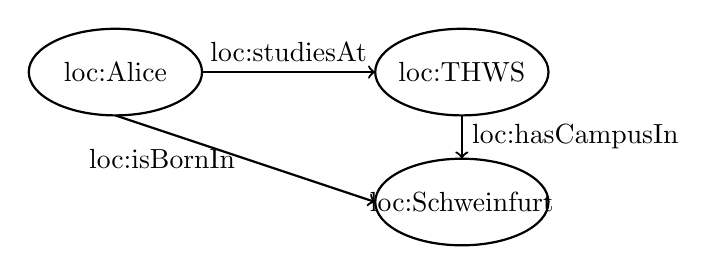
\begin{tikzpicture}[scale=0.55,thick]
	
		\draw (0,0) ellipse (2 and 1) node[] {\urisize loc:Alice};
		\draw[->] (2,0) -- (6,0)  node[midway,above] {\urisize loc:studiesAt};
		\draw (8,0) ellipse (2 and 1) node[] {\urisize loc:THWS};	
	
		\draw[->] (8,-1) -- (8,-2)  node[midway,right] {\urisize loc:hasCampusIn};
		\draw (8,-3) ellipse (2 and 1) node[] {\urisize loc:Schweinfurt};	

		\draw[thick,->] (0,-1) -- (6,-3) node[midway,left] {\urisize loc:isBornIn};
	\end{tikzpicture}
	\end{center}
	
	\textbf{Limitation of OWL (and other Description Logics)}
	\begin{itemize}
		\item Cannot represent the formula without enlarging the ontology
		\item Uncertainties are not supported in classical logics
	\end{itemize}
\end{frame}



\begin{frame}{$\sparql$ Queries }
	
The formula
	\begin{align*}
	 	\forall x,y,z: \big(
		\mathrm{studiesAt}(x,y) \cap & \mathrm{hasCampusIn}(y,z) \cap \mathrm{isBornIn}(x,z) \big) \\
		 & \rightarrow \mathrm{livesAtParents}(x) 
	\end{align*}
can be materialized by the $\sparql$ Query	
\begin{centeredscript}
INSERT\{ \\
\hspace{2cm} ?x  rdf:type  loc:livesAtParents . \\
\hspace{1cm} \} \\
\hspace{1cm}  WHERE\{ \\
\hspace{2cm} ?x  loc:studiesAt  ?y .\\
\hspace{2cm} ?y  loc:hasCampusIn ?z .\\
\hspace{2cm} ?x  loc:isBornIn  ?z .\\ 
 \hspace{1cm} \}
\end{centeredscript}
	

\end{frame}



\begin{frame}{Grounding Tensors}

Towards expressing $\sparql$ Queries in Tensor Networks

\begin{definition}[Grounding Tensor]
	Given a specific world $\worldvariables$, with a set of objects $\variableset$, the grounding of a formula $\exformula$ with $\individualorder$ arguments is the tensor
		\[ \groundingof{\exformula} :  \bigtimes_{\variableenumeratorin} \variableset \rightarrow [2] \]
	defined as
		\[ \groundingof{\exformula} \left(\individuals \right) = 
			\begin{cases}
				1 \quad \text{if $\exformula\left(\individuals\right)=1$ given the world $\worldvariables$}  \\
				0 \quad \text{else}
			\end{cases} \, . 
		\]
\end{definition}

\end{frame}



\begin{frame}{Knowledge Graphs as grounding tensors}

Knowledge Graphs $\kg$ are worlds $\worldvariables$, which are fully specified by the $\rdf$ formula.
Having a set of variables $\variableset$ we represent a Knowledge Graph $\kg$ by the tensor
\begin{align*}
	\kggroundingof{\rdf} : \variableset \times \variableset \times \variableset \rightarrow [2]
\end{align*}
where
\begin{align*}
	\kggroundingof{\rdf}(\variableof{s}, \variableof{p}, \variableof{o}) =
	\begin{cases}
	1 \quad & \text{if triple $\braket{\variableof{s}, \variableof{p}, \variableof{o}}$ is in Knowledge Graph $\kg$} \\
	0  \quad & \text{else}
	\end{cases} \, .
\end{align*} 


\begin{center}
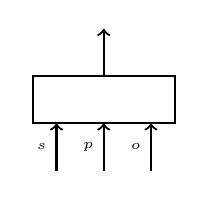
\begin{tikzpicture}[scale=0.3, thick] % , baseline = -3.5pt

    	\draw[->] (0,1)--(0,3); % node[midway,left] {\tiny $\atomicformula$};
    	\draw (-3,1) rectangle (3,-1);
	\node[anchor=center] (text) at (0,0) {\small $\kggroundingof{\rdf}$};
    	\draw[<-] (-2,-1)--(-2,-3) node[midway,left] {\tiny $\variableof{\sindex}$};
    	\draw[<-] (0,-1)--(0,-3) node[midway,left] {\tiny $\variableof{\pindex}$};
   	 \draw[<-] (2,-1)--(2,-3) node[midway,left] {\tiny $\variableof{\oindex}$};
\end{tikzpicture}
\end{center}

\end{frame}


\begin{frame}{Basic Graph Patterns}

Basic Graph Patterns are restrictions of the $\rdf$ formula on specific arguments, for example
\begin{itemize}
	\item Unary triple pattern with one variable, representing a formula with a single projection variable.
	 	For example: $\exunarytriple$ 
	\item Binary triple pattern with two variables, representing a formula with two projection variables.
		For example: $\exbinarytriple$ 
\end{itemize}

Their grounding tensors are slices of the $\rdf$

\begin{center}
\begin{tikzpicture}[scale=0.3,thick] % , baseline = -3.5pt

    \begin{scope}
        [shift={(0,0)}]

        \node[anchor=center] (text) at (-12,2) {$a)$};

        \begin{scope}
            [shift={(-7,2)}]

            \draw (0,-3) rectangle (-6,-5);
            \draw[-<-] (-3,-1)--(-3,-3) node[midway,right] {\colorlabelsize $\headvariable$};
            \node[anchor=center] (text) at (-3,-4) {$\bencodingof{\kggroundingof{\exunarytriple}}$};
            \draw[-<-] (-3,-5)--(-3,-7) node[midway,left] {\colorlabelsize $\provariableof{0}$};

        \end{scope}

        \node[anchor=center] (text) at (-5.5,-2) {${=}$};

        \draw[->-] (0,1)--(0,3) node[midway,left] {\colorlabelsize $\headvariable$};
        \draw (-4,1) rectangle (4,-1);
        \node[anchor=center] (text) at (0,0) {\corelabelsize $\bencodingof{\kggroundingof{\rdf}}$};

        \draw (-2,-3) rectangle (-4,-5);
        \draw[-<-] (-3,-1)--(-3,-3) node[midway,left] {\colorlabelsize $\sindvariable$};
        \node[anchor=center] (text) at (-3,-4) {$\delta$};
        \draw[-<-] (-3,-5)--(-3,-7) node[midway,left] {\colorlabelsize $\provariableof{0}$};

        \draw (-1,-3) rectangle (1,-5);
        \draw[-<-] (0,-1)--(0,-3) node[midway,left] {\colorlabelsize $\pindvariable$};
        \node[anchor=center] (text) at (0,-4) {$\onehotmapof{\invrdftypesymbol}$};

        \draw (2,-3) rectangle (4,-5);
        \draw[-<-] (3,-1)--(3,-3) node[midway,left] {\colorlabelsize $\oindvariable$};
        \node[anchor=center] (text) at (3,-4) {$\onehotmapof{\exaunaryrelation}$};

    \end{scope}


    \begin{scope}
        [shift={(24,0)}]

        \node[anchor=center] (text) at (-13,2) {$b)$};

        \begin{scope}
            [shift={(-8,2)}]

            \draw (0.5,-3) rectangle (-6.5,-5);
            \draw[-<-] (-3,-1)--(-3,-3) node[midway,right] {\colorlabelsize $\headvariable$};
            \node[anchor=center] (text) at (-3,-4) {$\bencodingof{\kggroundingof{\exbinarytriple}}$};

            \draw[-<-] (-2,-5)--(-2,-7) node[midway,right] {\colorlabelsize $\provariableof{0}$};
            \draw[-<-] (-4,-5)--(-4,-7) node[midway,left] {\colorlabelsize $\provariableof{1}$};

        \end{scope}

        \node[anchor=center] (text) at (-5.5,-2) {${=}$};

        \draw[->-] (0,1)--(0,3) node[midway,left] {\colorlabelsize $\headvariable$};
        \draw (-4,1) rectangle (4,-1);
        \node[anchor=center] (text) at (0,0) {\corelabelsize $\bencodingof{\kggroundingof{\rdf}}$};

        \draw (-2,-3) rectangle (-4,-5);
        \draw[-<-] (-3,-1)--(-3,-3) node[midway,left] {\colorlabelsize $\sindvariable$};
        \node[anchor=center] (text) at (-3,-4) {$\delta$};
        \draw[-<-] (-3,-5)--(-3,-7) node[midway,left] {\colorlabelsize $\provariableof{1}$};

        \draw (-1,-3) rectangle (1,-5);
        \draw[-<-] (0,-1)--(0,-3) node[midway,left] {\colorlabelsize $\pindvariable$};
        \node[anchor=center] (text) at (0,-4) {$\onehotmapof{\exabinaryrelation}$};

        \draw (2,-3) rectangle (4,-5);
        \draw[-<-] (3,-1)--(3,-3) node[midway,left] {\colorlabelsize $\oindvariable$};
        \node[anchor=center] (text) at (3,-4) {$\delta$};
        \draw[-<-] (3,-5)--(3,-7) node[midway,right] {\colorlabelsize $\provariableof{0}$};

    \end{scope}

\end{tikzpicture}
\end{center}

\end{frame}



\begin{frame}{Statistical Models of Knowledge Graphs}
	
	Limitation of Knowledge Graphs:
	\begin{itemize}
		\item Handling of \emph{Uncertainty}: How to reason given uncertain knowledge?
		\item \emph{Expressivity} of Logics: Which relations can be modelled?
	\end{itemize}
	
	\begin{columns}
		\column{0.35 \linewidth}
		\begin{center}
			\textbf{Knowledge Graph} \\
			{Data described in logics} \\
			Logical reasoning about \\ 
			\emph{connectivity}
		\end{center}
		\column{0.125 \linewidth}		
			\centering
			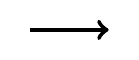
\begin{tikzpicture}
  				\draw[->, ultra thick] (0,0) -- (1,0);
			\end{tikzpicture}

		\column{0.475 \linewidth}
		\begin{center}
		\textbf{Statistical ("Graphical") Models} \\
			{Statistical dependencies of links} \\
			Probabilistic reasoning about \emph{samples}
		\end{center}
		
	\end{columns}

	\ \\ 
	
	\begin{block}{Connectivity to Samples: Towards building statistical models}
		\begin{itemize}
			\item Identify subgraphs of the Knowledge Graph to be interpreted as independent samples
			\item Learn and infer graphical models to reason about subgraphs
		\end{itemize}
	\end{block}

%	Techniques being applied:
%		\begin{itemize}
%			\item \emph{Tensorization}: Store truth of statements in sparse tensors 
%			\item \emph{Propositionalization}: Represent theory in propositional logics
%		\end{itemize}	
\end{frame}



\begin{frame}{Extraction of samples for statistical models}

The extraction is specified by
\begin{itemize}
	\item \textbf{Extraction query} $\exquery$ specifying the conditions on a pair of individuals to represent a sample
	\item \textbf{Atom queries} $\atomicqueryof{\atomenumerator}$ extracting the satisfaction of the atom for each pair of individuals 
\end{itemize}

By contraction we get an empirical distribution by
\begin{center}

\begin{tikzpicture}[scale=0.35, yscale=1, thick] % , baseline = -3.5pt


    \draw[->-] (2,-1) -- (2,1) node[midway,left] {\colorlabelsize $\catvariableof{0}$};
    \node[anchor=center] (text) at (4,0) {$\cdots$};
    \draw[->-] (6,-1) -- (6,1) node[midway,right] {\colorlabelsize $\catvariableof{\atomorder-1}$};

    \draw (1,-1) rectangle (7,-3);
    \node[anchor=center] (text) at (4,-2) {$\empdistribution$};
    \node[anchor=center] (text) at (-1,-2) {$\datanum \,\, \cdot $};

    \node[anchor=center] (text) at (10,-2) {${=}$};

    \begin{scope}
        [shift={(12,0)}]

        \draw[->-] (2.5,1) -- (2.5,3) node[midway,right] {\colorlabelsize $\catvariableof{0}$};
        \draw (1,-1) rectangle (4,1);
        \node[anchor=center] (text) at (2.5,0) {$\bencodingof{\groundingof{\extformulaof{0}}}$};
        \node[anchor=center] (text) at (2.5,-2) {$\cdots$};

        \node[anchor=center] (text) at (6.5,0) {$\cdots$};

        \draw[->-] (10.5,1) -- (10.5,3) node[midway,right] {\colorlabelsize $\catvariableof{\atomorder-1}$};
        \draw (8.75,-1) rectangle (12.25,1);
        \node[anchor=center] (text) at (10.5,0) {$\bencodingof{\groundingof{\extformulaof{\atomorder\shortminus1}}}$};
        \node[anchor=center] (text) at (10.5,-2) {$\cdots$};

        \draw[-<-] (13,-3) -- (3.5,-3) ;
        \draw[-<-] (13,-5) -- (1.5,-5) ;

        \drawvariabledot{11.5}{-3}
        \draw[->-] (11.5,-3) -- (11.5,-1);

        \drawvariabledot{9.5}{-5}
        \draw[->-] (9.5,-5) -- (9.5,-1);

        \drawvariabledot{3.5}{-3}
        \draw[->-] (3.5,-3) -- (3.5,-1);

        \drawvariabledot{1.5}{-5}
        \draw[->-] (1.5,-5) -- (1.5,-1);

        \draw (13,-2) rectangle (17,-6);
        \node[anchor=center] (text) at (15,-4) {$\bencodingof{\groundingof{\impformula}}$};
        \node[anchor=center] (text) at (12,-3.75) {$\vdots$};
        \draw[->-] (17,-4) -- (18,-4);
        \drawvariabledot{18}{-4}
        \draw[] (18,-4) -- (19,-4);
        \draw (19,-3) rectangle (21,-5);
        \node[anchor=center] (text) at (20,-4) {$\tbasis$};

    \end{scope}


\end{tikzpicture}
\end{center}

\end{frame}


\begin{frame}{Representation in Data Cores}

Having a CP Decomposition of $\kggroundingof{\exquery}$  we build datacores by
\begin{center}
\begin{tikzpicture}[scale=0.35, yscale=1, thick] % , baseline = -3.5pt


    \draw[->-] (4,-1) -- (4,1) node[midway, right] {\colorlabelsize $\catvariableof{\atomenumerator}$};
    \draw (3,-1) rectangle (5,-3);
    \node[anchor=center] (text) at (4,-2) {$\datacoreof{\atomenumerator}$};
    \draw[-<-] (4,-3) -- (4,-5) node[midway, right] {\colorlabelsize $\datvariable$};

    \node[anchor=center] (text) at (7,-2) {${=}$};

    \begin{scope}
        [shift={(10,0)}]

        \draw[->-] (3,1) -- (3,3) node[midway, right] {\colorlabelsize $\catvariableof{\atomenumerator}$};
        \draw (-1,1) rectangle (7,-1);
        \node[anchor=center] (text) at (3,0) {$\bencodingof{\groundingof{\extformulaof{\atomenumerator}}}$};

        \draw[->-] (0,-3) -- (0,-1) node[midway,left] {\colorlabelsize $\indvariableof{0}$};
        \draw[->-] (3,-3) -- (3,-1) node[midway,left] {\colorlabelsize $\indvariableof{1}$};
        \draw[->-] (6,-3) -- (6,-1) node[midway,left] {\colorlabelsize $\indvariableof{2}$};


    \end{scope}

    \begin{scope}
        [shift={(10,-2)}]

        \coordinate (conposseldec) at (4.5,-5.5);
        \drawvariabledot{4.5}{-5.5}
        \draw[-<-] (conposseldec) -- (4.5,-7.5) node[midway, right] {\colorlabelsize $\indexvariable$};

        \draw (-1,-1) rectangle (1, -3);
        \node[anchor=center] (text) at (0,-2) {\corelabelsize $\bencodingof{\secdatamap_0}$};%{\corelabelsize $\legcoreof{\fixedimpformula,0}$};
        \draw[-<-] (0,-3) to[bend right=20] (conposseldec);

        \draw (2,-1) rectangle (4, -3);
        \node[anchor=center] (text) at (3,-2) {\corelabelsize $\bencodingof{\secdatamap_1}$};%{\corelabelsize $\legcoreof{\fixedimpformula,1}$};
        \draw[-<-] (3,-3) to[bend right=20]  (conposseldec);

        \draw (5,-1) rectangle (7, -3);
        \node[anchor=center] (text) at (6,-2) {\corelabelsize $\bencodingof{\secdatamap_2}$};%{\corelabelsize $\legcoreof{\fixedimpformula,2}$};
        \draw[-<-] (6,-3) to[bend right=-20]  (conposseldec);

        \draw[-<-] (9,1) -- (9,-1) node[midway,left] {\colorlabelsize $\indvariableof{3}$};
        \draw (8,-1) rectangle (10, -3);
        \node[anchor=center] (text) at (9,-2) {\corelabelsize $\bencodingof{\secdatamap_3}$};%{\corelabelsize $\legcoreof{\fixedimpformula,3}$};
        \draw[-<-] (9,-3) to[bend right=-20]  (conposseldec);


        \node[anchor=center] (text) at (12,-2) {$\cdots$};

        \draw[-<-] (15,1) -- (15,-1) node[midway,left] {\colorlabelsize $\indvariableof{\indorder-1}$};
        \draw (13.5,-1) rectangle (16.5, -3);
        \node[anchor=center] (text) at (15,-2) {\corelabelsize $\bencodingof{\secdatamap_{\indorder-1}}$};%{\corelabelsize $\legcoreof{\fixedimpformula,\variableorder-1}$};
        \draw[-<-] (15,-3) to[bend left=20]  (conposseldec);


        \draw (8,1) rectangle (16, 3);
        \node[anchor=center] (text) at (12,2) {\corelabelsize $\ones$};


    \end{scope}


    \node[anchor=center] (text) at (29,-2) {${=}$};


    \begin{scope}
        [shift={(32,0)}]

        \draw[->-] (3,1) -- (3,3) node[midway, right] {\colorlabelsize $\catvariableof{\atomenumerator}$};
        \draw (-1,1) rectangle (7,-1);
        \node[anchor=center] (text) at (3,0) {$\bencodingof{\groundingof{\extformulaof{\atomenumerator}}}$};

        \draw[->-] (0,-3) -- (0,-1) node[midway,left] {\colorlabelsize $\indvariableof{0}$};
        \draw[->-] (3,-3) -- (3,-1) node[midway,left] {\colorlabelsize $\indvariableof{1}$};
        \draw[->-] (6,-3) -- (6,-1) node[midway,left] {\colorlabelsize $\indvariableof{2}$};


    \end{scope}

    \begin{scope}
        [shift={(32,-2)}]


        \coordinate (conposseldec) at (3,-5.5);
        \drawvariabledot{3}{-5.5}
        \draw[-<-] (conposseldec) -- (3,-7.5) node[midway, right] {\colorlabelsize $\datvariable$};

        \draw (-1,-1) rectangle (1, -3);
        \node[anchor=center] (text) at (0,-2){\corelabelsize $\bencodingof{\secdatamap_0}$};%{\corelabelsize $\legcoreof{\fixedimpformula,0}$};
        \draw[-<-] (0,-3) to[bend right=20] (conposseldec);

        \draw (2,-1) rectangle (4, -3);
        \node[anchor=center] (text) at (3,-2) {\corelabelsize $\bencodingof{\secdatamap_1}$};%{\corelabelsize $\legcoreof{\fixedimpformula,1}$};
        \draw[-<-] (3,-3) to[bend right=0]  (conposseldec);

        \draw (5,-1) rectangle (7, -3);
        \node[anchor=center] (text) at (6,-2) {\corelabelsize $\bencodingof{\secdatamap_2}$};%{\corelabelsize $\legcoreof{\fixedimpformula,2}$};
        \draw[-<-] (6,-3) to[bend right=-20]  (conposseldec);


    \end{scope}


\end{tikzpicture}
\end{center}
and have a representation 
\begin{align*}
	\datanum \cdot \contractionof{\empdistribution}{\enumeratedatoms} = \contractionof{\datacoreof{0},\ldots,\datacoreof{\atomorder-1}}{\enumeratedatoms} \, .
\end{align*}

This amounts to a CP Decomposition of $\empdistribution$, which \textbf{can introduce storage overheads}!

\end{frame}


\begin{frame}{Statistical Models of Knowledge Graphs}

\textbf{Learning}:
\begin{itemize}
	\item Extract samples based on the extraction query and the atom queries
	\item Train a Markov Logic Model based on neuro-symbolic architectures and parameter estimation
\end{itemize}

\medskip

\textbf{Inference}:
\begin{itemize}
	\item Estimate the probability of missing links (by modification of atom truths)
	\item Generate Knowledge Graphs based on samples of the statistical model
\end{itemize}

\end{frame}

\end{document}